
\documentclass[a4paper]{article}

\usepackage[english]{babel}
\usepackage[utf8]{inputenc}
\usepackage{amsmath}
\usepackage{graphicx}
\usepackage[colorinlistoftodos]{todonotes}
\usepackage{float}
\usepackage{hyperref}
\usepackage{multicol}
\setlength\parindent{0pt}

\title{Footpath Planning for Example-driven Procedural Road Networks}

\author{Alexander Hjelm}

\date{\today}

\begin{document}
\maketitle

\section{Abstract}

\begin{figure}[H]
\centering
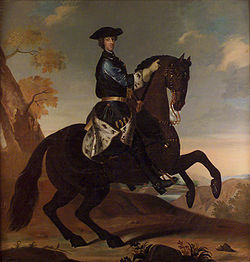
\includegraphics[height=0.5\textheight]{test_image}
\caption{En typisk rymdhiss enligt Wikipedia. Bildkälla (\cite{sampleitem1}).}
\label{fig:space}
\end{figure}

This report covers... \cite{sampleitem2}

\section{Introduction}

\subsection{Research Question}

This research question deals with the procedural generation of road networks from example data sets, and the edge cases that arise when dealing with footpath planning. A common problem is that footpaths are in their nature placed densely. How can the program identify critical areas where the footpath width is so large that it collides with existing roads? Can this be done so efficiently that the example-driven program can still run in real time? An additional question that arises is how much road data will be necessary to create believable procedural road networks for new zones in the Stockholm metropolitan area. How can this data be sampled and processed efficiently?

The previous work by Nishida et. al. has shown that it is possible to create believable procedural road maps from examples. Their program has created a network of 35 km road in less than a second, so for the application of zoning new city areas my hypothesis is that such a program can be made to run in real time with such minimal waiting time that it can be used in a real application by a city planner.

The challenge lies in how to extract the footpath data and tie it together with the existing road map. the work by Nishida et. al. only deals with arterial and secondary roads, and I will be adding a tertiary layer of roads, wich is highly possible, but may increase the data consumption and program running time. The same applies for the statistical model that identifies colliding roads, which I will be adding on top of that.

\subsection{Problem Constraints}

\begin{enumerate}
\item The road network is assumed to be a 2D simple graph. This means that any overlapping roads, such as tunnels and bridges that cross over street-level roads, will be eliminated from the training set. Any self-connected nodes will also be eliminated from the training set.
\item It will be assumed that the city map consists of only arterial (primary) roads, secondary roads and footpaths.
\item It will be assumed that the primary, secondary and tertiatry roads all have a fixed width. Primary roads have a set width, and secondary roads and footpaths as well.
\item It will be assumed that the use case of the application is for generating areas with the size of a neighbourhood or a few city blocks. The area that the user will sketch will typically be around 0.1 km2.
\item The program will not handle terrain features and altitude. It will be assume that the road mesh is projected on a flat 2D surface.
\end{enumerate}

With that said, Nishida et. al. present an excellent solution for generating new road patches that comform to an underlying terrain function.

\subsection{Evaluation}

The question will be examined primarily by creating a piece of software that can generate urban maps with primary and secondary roads, as well as footpaths, from example. I will experiment with different methods of collecting road data as well as different sample amounts and densities.

The evaluation plan will consist of programmatic evaluations and quantifyable metrics. My main idea is to sample metrics about intersections only (number of connecting roads, the angles between them, distance to connecting intersections, curviness of roads, etc). If I can sample all that and create a distribution for a few different cities, I have the two following hypothesises:
  1. There should be selection of features that produce an observable difference in the distributions between cities that look vastly different.
  2. If I let my program generate a large number of city parcels from a dataset, the resulting feature distribution should look like to the source dataset, and unlike datasets of other cities.
These distributions could be created for primary, secondary roads and footpaths separately.

\subsection{Background}

Procedural modeling of road networks is of interest to the fields of urban planning and urban architecture. In recent years there has been an advent of interactive tools that aid urban planners in placing or generating features of an urban plan, particularly roads and road networks.
Additionally, the topic is of interest for 3D content creators in for example the fields of video game design or 3D animation. A trend in these fields is using methods of procedural modeling to create large amounts of 3D content quickly and efficiently, while requiring as little hand modeling as possible. Studios who create large worlds are often interested in solutions that generate large road networks without any hand modeling.

Motivation

Navigation agents, they might fail navigating when faced with a too narrow path or intersecting obstacles
Using a road network to creates an underlying navmesh

\subsection{ESAL, KTH}
The thesis work will be carried out at the Embodied Social Agents Lab (ESAL) at the Department of Computational Science and Technology (CST). The lab has before been working on systems for generating procedural urban environments, and are interested in the possibility of generating more detailed maps than have been done before, using example-based methods to preserve the aesthetic look of a greater metropolitan area. The lab is particularly interested in the generation of footpaths, since most commercial software that import road maps only import arterial and secondary car roads, and do not include pedestrian walkways, cycle paths and such smaller roads.
% TODO: any official description of ESAL that can be used here?

\section(OSM Data)

To separate sidewalks from detached footpaths, I used the fact that OSM generally provides sidewalks with the same name as the adjacent motorway. Thus they can be paired together and measured against each other.

\subsection(SLU Data)

The SLU map is maintained by The Swedish National Land Survey (Swedish: Lantmäteriet).
The SLU data is aqqcuired by land surveying methods such as GPS or DGNSS positioning, or by reproduction of features from ortophoto or stereo mapping from 3D aerial images.
The map is updated continously by Lantmäteriet, in conjoncture with the forming or reforming of property.
Property limits and building features have a position accuracy requirement of 5 meters.
(Lantmäteriet, 2019)

\subsection(A word on coordinate systems)

The SLU dataset comes in the SWEREF 99 TM (Lantmäteriet, 2019). SWEREF 99 TM is a projected coordinate system and there is no linear transformation to WGS 48, which OpenStreetMap uses (OSM 19). The coordinate conversions for this paper were obtained using proj: a Linux commandline application for geospatial coordinate conversion.

\section{Implementation}

In this implementation, roads of different types were allowed to merge into one another to form common intersections. To facilitate this, it was neccessary to work with a path-by-path representation of the point data. When two path share a node with common coordinates, they form an intersection which can be of multiple different types.

\begin{thebibliography}{9}

\bibitem{lantmateriet-19}
(Lantmäteriet, 2019), Produktbeskrivning: GSD-Fastighetskartan vektor \\ 
\href{https://www.lantmateriet.se/globalassets/kartor-och-geografisk-information/kartor/fastshmi.pdf}.

\bibitem{osm-19}
(OSM 19) Converting to WGS84, accessed 13-03-2020\\ 
\href{https://wiki.openstreetmap.org/wiki/Converting_to_WGS84}.

\end{thebibliography}


\end{document}
